%\begin{flushright}
%\end{flushright}
\documentclass{template/openetcs_report}
% Use the option "nocc" if the document is not licensed under Creative Commons
%\documentclass[nocc]{template/openetcs_article}
\usepackage{lipsum,url}
\usepackage{supertabular}
\usepackage{multirow}
\usepackage{color, colortbl}
\usepackage{float}
\definecolor{gray}{rgb}{0.8,0.8,0.8}
\usepackage[modulo]{lineno}
\usepackage{comment}
\graphicspath{{./template/}{.}{./images/}}


%=======================================================================
%%%%% comments %%%%%
% To allow MS Word style comments at the document margin we use the todonotes package. A comment is made as follows:

%\mycomment[IN]{text}

% The text in brackets should be your initials and the text in curly braces is your actual comment. Comments are numbered automatically. 
\usepackage[textwidth=2.7cm,textsize=scriptsize,linecolor=green!40,backgroundcolor=green!40]{todonotes}

\newcounter{mycommentcounter}
\newcommand{\mycomment}[2][]
{
\refstepcounter{mycommentcounter}%
\todo[color={red!100!green!33}]{
\textbf{[\uppercase{#1} \themycommentcounter]:} #2}
}
\setlength{\marginparwidth}{2.5cm}
%\reversemarginpar
%=======================================================================


\begin{document}
\frontmatter
\project{openETCS}

%Please do not change anything above this line
%============================
% The document metadata is defined below

%Background color of boxes in process graphic
\definecolor{light-gray}{gray}{0.95}

%assign a report number here
\reportnum{OETCS/WP2/D2.3b}

%define your workpackage here
\wp{Work-Package 2}

%set a title here
\title{Scrum Process in openETCS Project}

%set a subtitle here
\subtitle{}

%set the date of the report here
\date{August 2015} % \\ Revised April 2015}

%document approval
%define the name and affiliation of the people involved in the documents approbation here
\creatorname{Abdelnasir Mohamed}
\creatoraffil{AEbt}

\techassessorname{}
\techassessoraffil{}

\qualityassessorname{}
\qualityassessoraffil{}

\approvalname{Klaus-R\"udiger Hase}
\approvalaffil{DB Netz}

%define a list of authors and their affiliation here

\author{Abdelnasir Mohamed}

\affiliation{AEbt Angewandte Eisenbahntechnik GmbH\\
  Adam-Klein-Str. 26 \\
  90429 Nürnberg, Germany\\
  eMail: abdelnasir.mohamed@aebt.de \\
  WebSite: www.aebt.de}  

\author{Jan Welte}

\affiliation{Technische Universität Braunschweig\\
  Institute for Traffic Safety and Automation Engineering\\
  Hermann-Blenk-Str. 42\\
  38108 Braunschweig, Germany\\
  eMail: openetcs@iva.ing.tu-bs.de \\
  WebSite: www.iva.ing.tu-bs.de}
  

%add yourself as author, if you contributed to the document



% define the coverart
\coverart[width=350pt]{openETCS_EUPL}

%define the type of report
\reporttype{Output Document}


\begin{abstract}

\end{abstract}

%=============================
%Do not change the next three lines
\maketitle
\tableofcontents
\listoffiguresandtables
\newpage
%=============================

\chapter{Document Control}

\begin{tabular}{|p{4.4cm}|p{8.7cm}|}
\hline
\multicolumn{2}{|c|}{Document information} \\
\hline
Work Package &    \\
Deliverable ID & \\
\hline
Document title & openETCS \\
Document version & 0.3 \\
Document authors (org.)  & Jan Welte (TU-BS) and Abdelnasir Mohamed (AEbt)\\
\hline
\end{tabular}

\begin{tabular}{|p{4.4cm}|p{8.7cm}|}
\hline
\multicolumn{2}{|c|}{Review information} \\
\hline
Last version reviewed & 0.1 \\
\hline
Main reviewers (org.) & \\
\hline
\end{tabular}

\begin{tabular}{|p{2.2cm}|p{4cm}|p{4cm}|p{2cm}|}
\hline
\multicolumn{4}{|c|}{Approbation} \\
\hline
  &  Name & Role & Date   \\
\hline  
Written by    &  Jan Welte & WP4-T4.4 Task Leader  &  November 2015\\
\hline
Approved by & -- & -- & \\
\hline
\end{tabular}

\begin{tabular}{|p{2.2cm}|p{2cm}|p{4cm}|p{4cm}|}
\hline
\multicolumn{4}{|c|}{Document evolution} \\
\hline
Version &  Date & Author(s) & Justification  \\
\hline
0.1 & 18/08/2015 & Jan Welte &  Document creation \\
\hline 
0.2 & 19/10/2015 & Abdelnasir Mohamed & Chapter 1.1 \\
\hline  
0.3 & 28/01/2014 & Jan Welte & Editing of Chapter 1.2, 3 and 4  \\

\hline  
\end{tabular}
\newpage

%=========ToDo List===========
%\listoftodos[ToDo List]
%\newpage
% The actual document starts below this line
%=============================

\mainmatter

\chapter{Introduction}
\label{sec:introduction}

\begin{comment} 
Nasir

Short introduction to this document.
\mycomment[AM]{Introduction: finish section writing}
\begin{itemize}
\item extension to QA-Plan and Process Description
\end{itemize}
\end{comment}


\section{Purpose}
\label{sec:purpose}

The purpose of this document is to define and describe the agile work-flow of the software development process in the openETCS project. As the outcomes of the project, the openETCS software and the openETCS development tool chain, are precisely defined, the process of how these two artifacts at the beginning of the development process are being produced in detail is not clear. In the conventional software development  process, e.g. with a V-Model, the life cycle of the development is implemented in closed non re-definable phases, which they shall be processed consecutively. 

Due to the complex nature of the openETCS as a  Research and Development (R\&D) Project an agile methodology is needed, which it's framework facilitates continuous refinements and improvements throughout the whole openETCS software development process. In this agile way of development complex tasks are broken down into smaller tasks (increments), which shall be executed in short time frames called Sprints. This document will be describing the agile framework in openETCS development process applying SCRUM.


%\section{Document Structure}
%\label{sec:document-structure}



%\section{Document Evolution}



\section{Reference Documents}
\label{sec:refdoc}

This document essentially refers to the following standards, ETCS specification documents and openETCS project documents.

\begin{itemize}
\item \textbf{ISO~9000} --- 12/2005 --- \emph{Quality management}
\item \textbf{ISO~9001} --- 12/2008 --- \emph{Quality management systems — Requirements}
\item \textbf{ISO~25010} --- 03/2011 --- \emph{Systems and software engineering -- Systems and software Quality Requirements and Evaluation (SQuaRE) -- System and software quality models}
\item \textbf{CENELEC EN~50126-1} --- 01/2000 --- \emph{Railways applications –- The specification and 
demonstration of Reliability, Availability, Maintenability and Safety (RAMS) –- Part 1: 
Basic requirements and generic process}
\item \textbf{CENELEC EN~50128} --- 10/2011 --- \emph{Railway applications -- Communication, signalling and 
processing systems -- Software for railway control and protection systems}
\item \textbf{CENELEC EN~50129} --- 05/2003 --- \emph{Railway applications –- Communication, signalling and 
processing systems –- Safety related electronic systems for signalling}
\item \textbf{CCS~TSI} --- \emph{ CCS TSI for HS and CR transeuropean rail has been adopted by a Commission Decision 2012/88/EU on the 25th January 2012}
\item \textbf{SUBSET-026} 3.3.0 --- \emph{System Requirement Specification}
\item \textbf{SUBSET-091} 3.2.0 --- \emph{Safety Requirements for the Technical Interoperability
of ETCS in Levels 1 \& 2}
\item \textbf{SUBSET-088} 2.3.0 --- \emph{ETCS Application Levels 1 \& 2 - Safety Analysis}
\item \textbf{OpenETCS FPP} --- \emph{Project Outline Full Project Proposal Annex OpenETCS} -- v2.2
\item \textbf{OpenETCS D2.2} -- Report on CENELEC standard
\item \textbf{OpenETCS D2.3} -- Definition of the overall process for the formal description of ETCS and the rail system it works in 
\item \textbf{OpenETCS D2.4} -- Definition of the methods used to perform the formal description
\item \textbf{The Scrum Guide} -- The Definitive Guide to Scrum: The Rules of the Game, July 2013
\end{itemize}


%%%%%%%%%%%%%%%%%%%%%%%%%%%%%%%%%%%%%%%%%%%%%%%%%%%%%%%%%%%%%%%

\section{Glossary}
\label{sec:glossary}



\begin{tabular}{rl}
%\textbf{ACedit} & Assurance Case Editor \\ 
\ %textbf{ARM} & Argumentation  Metamodel \\ 
\textbf{ETCS} & European Train Control System \\ 
\textbf{ERA} & European Railway Agency \\ 
\textbf{EVC} & European Vital Computer \\
\textbf{FMEA} & Failure Mode Effect Analysis \\ 
%\textbf{GSN} & Goal Structured Notation \\ 
%\textbf{MoRC} & Management of Radio Communication \\
\textbf{OBU} & On-Board Unit \\ 
\textbf{QA} & quality assurance \\
%\textbf{RAMS} & Reliability, Availability, Maintainability and Safety \\
\textbf{SIL} & Safety Integrity Level \\ 
\textbf{SRS} & System Requirement Specification \\ 
%\textbf{THR} & Tolerable Hazard Rate \\ 
\textbf{V\&V} & Verification \& Validation \\ 
\end{tabular} 




\section{Background Information}
\label{sec:Background}


\subsection{Agile Development}

At the beginning of the 1990s software developers started to see the traditional software development methods as inadequate and too inflexible to deal with the increasing dynamic environment. The development methods derived under this concept are today referred to as agile methods. The word agile is in this context understood in the sense of movable or nimble. 

The basic concept is to have a software development process, which is able to adapt to changing requirements from needs and wishes of the client while - or perhaps on these grounds - having a stable development. The traditional methods are based on the premise,that once a system has been specified and designed it can be implemented without major modifications. In accordance the requirements are collected as first as detailed as possible. Afterwards, a number of predefined artifacts is created in consecutive phases to increase the granularity up to the source code. In an agile understanding the empirical development process should be defined only as strict and distinct as it appears necessary and appropriate to ensure the project's success. By doing so agile software development implicitly address quality assurance (QA) through  continuous feedback and recurrent tests carried out during the development. In contrast, the QA is explicitly achieved through process standardization and testing in the traditional software development.

Each agile method applies in their own way steps to allow learning and to adopted changes. The various agile methods or their process models present themselves thereby not uniform as they differ considerably in their conceptions. Established agile methods are Adaptive Software Development, Extreme programming or Scrum. The openETCS project bases it's agile development on the SCRUM concept, which was devised in the 1990s by Ken Schwaber and Jeff Sutherland and uses ideas the lean production concept. The following subsection introduces the fundamental principals and roles of SCRUM.


\subsection{SCRUM Definition And Roles}

This section should be considered as an introduction for the following chapters to fit the content of this document. For more detailed information about SCRUM the \textit{Scrum Guide} is advisable to read. In the SCRUM Guide developed by Ken Schwaber and Jeff Sutherland, Scrum is defined as "\textit{A framework within which people can address complex adaptive problems, while productively and creatively delivering products of the highest possible value}". It is "\textit{simple to understand}" but "\textit{difficult to master}".

SCRUM defines three roles; the Product Owner (PO); the SCRUM Master (ScM) and the Development Team. All three roles together make the SCRUM Team.

\subsection{General SCRUM Framework}

Scrum process starts with a Product Backlog (PB), this Product Backlog contains an ordered list of requirements that is maintained for a product. The Product Backlog Items (PBIs) are ordered by the Product Owner based on considerations like risk, business value, date needed, etc. The Product Owner is the responsible of the product backlog and the prioritization of PBIs.

After the defining of the Product Backlog the next task is to create the Sprint planning meeting. This meeting is organized at the beginning of the Sprint cycle. The objective of this meeting is to define the PBIs to be done in following Sprint. The Sprint is the time period in which development occurs on a set of backlog items that the team has committed to (also commonly referred to as iteration). 

The result of PBIs selected for implementation in one Sprint is called the Sprint Backlog. The Sprint Backlog is the list of work the Development Team must address during the next Sprint. This list is derived by selecting product backlog items from the top of the product backlog until the Development Team fills it's capacity and make sure it has enough work to during the CompSprint.

Each day during the Sprint, a project team communication meeting occurs. This is called a daily Scrum Meeting and has specific guidelines. The Scrum Meeting is organized by the Scrum Master and the participants respond to three questions:
\begin{enumerate}
\item  What have you done since yesterday?
\item What are you planning to do today? 
\item And Any impediments/stumbling blocks?.
\end{enumerate}
At the end of the Sprint, the result of the PBIs implemented is called the increment (potentially shippable increment), this is the sum of all the Product Backlog items completed during a Sprint and all previous Sprints. The increment must be in a usable condition regardless of whether the Product Owner decides to actually release it.

At the end of Sprint cycle or iteration, two meetings are held; the Sprint review meeting and Sprint retrospective. The approximate duration of the spring review meeting will be no more than 4 hours and it will be moderated by the Scrum Master (ScM). In this meeting two main activities will take place. One is to review the the planned work that has been completed from the one that wasn't. And the second activity is to present to the Product owner the work done. The other meeting after iteration is the spring retrospective. This meeting will be moderated by the scrum master and it's main objective is the continuous process improvements. Two main questions are asked to all participants in this meeting:
\begin{itemize}
\item   what went well during the Sprint? 
\item What could be improved in the next Sprint?
\end{itemize}


\chapter{Agile Development in openETCS}
\label{sec:agile}

The openETCS Project is concerned with the development for the kernel software of an ETCS on-board unit (OBU). The European Vital Computer (EVC) as the central part ot the OBU contains the core control functionality fore the train movement and therefore has a SIL 4 classification according to the applicable CENELEC standards. Respectively, it software development has to satisfy the SIL 4 process requirements of the EN 50128 standard. 

Although the openETCS project itself only aims to provide a non vital functional reference implementations, which itself does not require SIL 4 methods, the project has the goal to provide a development methodology applicable for SIL 4 development. This process makes use of model-based development and agile development principals, while following the QA principals which are emphasized by the EN 50128 lifecycle. 

As the CENELEC standards have been defined based on a traditional V-Model development process, agile SCRUM principles are integrated in the openETCS development process by addressing tasks of several phases at the same time and thereby creating artifacts in an iterative steps. In addition the required organizational structures for SIL 4 development mainly ensuring independence between design, testing and V\&V have to be established in the agile work organization.

\section{Roles and Responsibilities}

Although the CENELEC standards and the SCRUM development process both define specific roles these have a different focus. The CENELEC roles are specified to establish responsibilities which are going along with specific tasks. The clear separation of certain roles between different personal which can also be under different organizational structures shall ensure Independence as the basis for QA. SCRUM roles are purely defined from a process view. They shall ensure that the costumer needs are always the focus point of all activities and that the agile principals of learning and adopting are always applied in a consistent way. Consequently, these roles for the most part are not separating working tasks performed during the development.
Therefore the QA aspect of the CENELEC roles can be fulfilled in a SCRUM working process by ensuring the required personal and organizational independence during the SCRUM work allocation. As the SCRUM process is focused on small communicating teams, it is reasonable to further strengthen the personal independence by addressing larger work portions like validation in separate SCRUM teams. By having several SCRUM Teams working a means has to be established to continuously allocate and groom the task between those teams and to incorporate the lessons learned. The openETCS project uses a so called SCRUM of SCRUM in which a representative of each SCRUM Team and the overall product owner pre-groom task and allocate them between the SCRUM Teams e.g. modling and V\&V. Afterwards each SCRUM teams grooms all tasks further and addresses them in their Sprint planning. Feedback from the Sprint review is channeled back tot the SCRUM of SCRUM if necessary. Only in the SCRUM Team specific people are assigned to as tasked in accordance with their qualification, which can provide the same separation and qualification assurance as required in a SIL 4 development.   
 
\section{Lifecycle}
The SCRUM process corresponding to the agile development principals does not explicitly defines artifacts which have to be delivered during the software lifecycle. The SCRUM process only provides a process framework in which all needed artifacts to satisfy costumer needs shall be developed and maintained. In contrast is the CENELEC lifecycle explicitly stating number of artifacts which shall be provided during the lifecycle. Respectively, these artifacts are provided during the openETCS development as it is presented in D2.3a and figure~\ref{fig:lifecycle2}. 

\begin{figure}[hbt]
  \centering
  \def\svgwidth{.9\textwidth}
  {\tiny
  \input{./images/Prcss2_3a-03.pdf_tex}}
  \caption{openETCS Development Lifecycle}
  \label{fig:lifecycle2}
\end{figure}


The agile development is applied as these artifacts are not produced one by one and without exchanges. In fact the artifact are more or less a result of tasks essential to reach the final goal of a functional ETCS OBU kernel software. All artifacts defined in D2.3 are either an intermediate product like the SysML Architecture Model or the SCADE Software Specification Model, or they are needed documentation and results for QA measures like plans and reports.

As the agile development is based on continues development, which repeatedly taken feedback and changes into account, the artifacts are completed over time with the ongoing work. Thereby, the system is developed in iterations, which has the consequence that also the corresponding artifacts are produced over time. Thereby, each iteration strongly requires V\&V steps for every artifact and simulation to allow costumer feedback. These QA measures are consistent with the CENELEC lifecycle principal which require verification and testing reports for every artifact and validation for the overall system. The critical step for the agile development is to ensure consistency between all related artifacts and to establish a capable configuration management to ensure that all findings and the resulted changes are taken into account properly in all following iterations. To allow fast feedback and be able to repeated these activities with every iteration a efficient tool support and test automation is needed in agile development. Figure~\ref{fig:openETCSSCRUMSprint} demonstrates the general SCRUM concept in openETCS.

\begin{figure}[hbt]
\centering
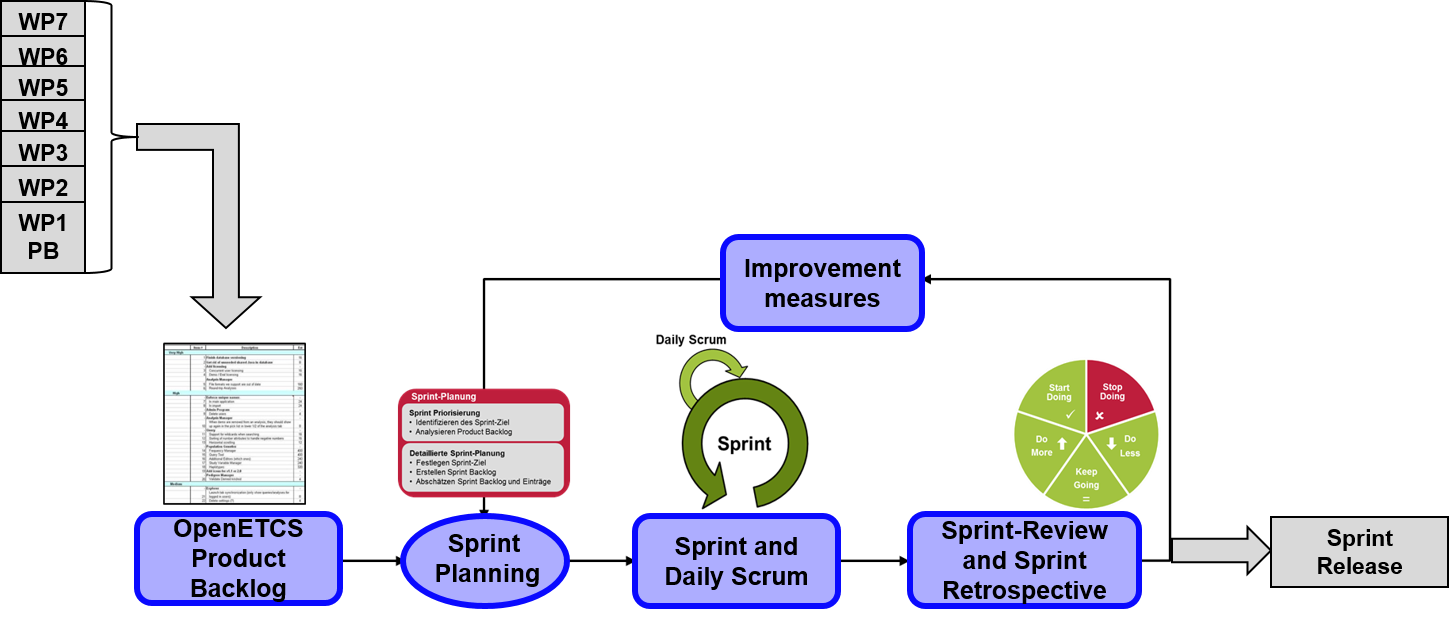
\includegraphics[width=0.95\linewidth]{./images/openETCSoverallScrum}
\caption{openETCS SCRUM Sprint}
\label{fig:openETCSSCRUMSprint}
\end{figure}

Since the V\&V activities are extensive for SIL 4 development the openETCS development separated simple test done by the development SCRUM Team itself and the independent V\&V checks performed by the V\&V SCRUM team. There interaction is coordinated through the SCRUM of SCRUM and releases as shown in section \ref{sec:Releases}.

On the whole the openETCS development process follows the EN 50128 V-model lifecycle for railway software development by using SysML and SCADE models as the man means of transcriptions during the development. Respectively, the EN 50128 artifacts are matched to these model-based design as presented in D2.3a. The agile process of SCRUM is applied to  develop these artifacts in incremental steps which changes the content in iterations. The basic relation between the artifacts and corresponding tasks follow the CENELEC QA concept.


\chapter{openETCS SCRUM Process}
\label{sec:ScrumProzess}

In openETCS there are three levels of processes that apply SCRUM:
\begin{itemize}
	\item The first level is the openETCS Project level, where Project Coordinator is the Product Owner. In this level the SCRUM meetings are organized every Friday.
	\item The second level is the Work Package level, where Work Package Leader is the Product Owner. In this level SCRUM meeting depends on WP, but at least two SCRUM meetings are organized every week.
	\item The last level is the Task level, where the Task Leader is the Product Owner. In this level SCRUM meeting period is variable and depends on the task.
\end{itemize}

\begin{figure}[h]
	\centering
	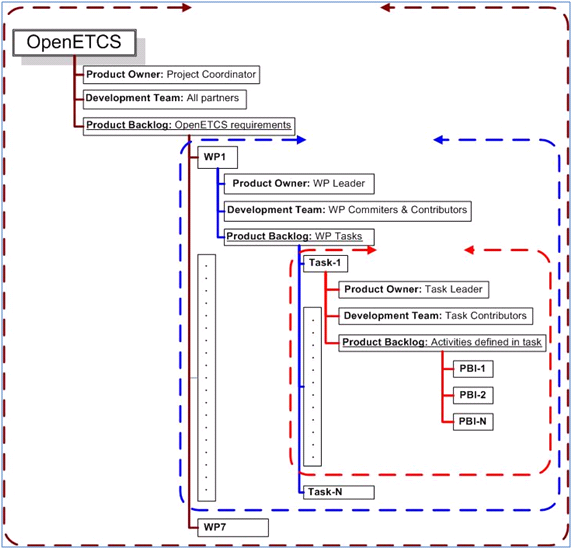
\includegraphics[scale=0.6]{./images/openetcs__scrum.png}
	\caption{openETCS Project Structure}
\end{figure}

\begin{comment}
\mycomment[AM]{finish section writing} \\
\end{comment}

\section{SCRUM Process in Work Packages}

\begin{comment}
- As defined in FPP there are 7 WPs\\
- WP Roles and it's conventions to conform the EN 50128 Roles\\
- Grafik of Roles for SW dev. in EN 50128 
- Every WP has its own PO\\
- Webbased CM (GitHub)\\
-----------------------------------------
\end{comment}

\textbf{Product backlog of the Modeling Team (WP3)}

The product backlog is implemented via the issue tracker.
The product backlog consists ofUse Cases, marked with the label "US-Operational Scenarios on Utrecht Amsterdam".
Each Use Cases has an unique User Story label identifing this Use Case in the backlog.
(Sub-) User Stories identified as necessary for the implementation of a Use Cases are marked with the user story label,

The actual work at the user stories is broken down in smaller technical tasks. These tasks are organised in the sprint backlog. Use the label sprint backlog for defining a task.
Remark: We will use specific sprint labels when we better start to organise the work in individual sprints.

The sprint backlog consists of prioritized tasks. Priorities are integers in the interval [1...1000], with 1000 representing the highest priority. Note that the absolute value is of minor interest, priorization is only needed to classify backlog items by importance.

Priorities are captured in the title of each task respectively issue. Example: US-SpeedMonitoring: Dynamic ASave Calculation Prio: 500 represents a user story with priority 500. The reason to capture the priority in the title is to make priority changes traceable, as the text of github issues may be changed without leaving any trace.

The labels Ready, In Progress, and Deferred are used to capture the state of user stories. Note that closing an issue is equivalent to the state Done.

A user story may only be moved to the state Ready when:
	A priority has been assigned.
	The scope is clearly defined and distinguished from other user stories in the states Ready or in Progress.
	The criteria for reaching the state Done are clear.
	When setting a user story to "done" a comment is mandatory for documenting the result.
	Every project member is eligible to propose user stories.

New user stories shall remain in the state (respectively column) Inbox until they have been reviewed by the team in a grooming session. 


\begin{comment}

\missingfigure{SCRUM in WPs} \\ \\


%mycomment{} have been wrongly placed on the left margin

Here!
\reversemarginpar
\mycomment[AM]{SCRUM in WPs GitHub: finish section writing}

\end{comment}

\section{Scrum of Scrums}

\begin{comment}
Nasir

Short introduction to principle of splitting work between different teams, as required by the EN 50128

Principles of grooming work and filling backlogs for distributed Scrum Teams by dynamic work allocation.

\end{comment}

%Text based on wiki page by Marc Behrens
%\mycomment[AM]{SCRUM of SCRUMS Wiki in WP3 GitHub: finish section writing}
%\textit{Objective:} 
Ongoing verification and validation of openETCS development artifacts are performed within the framework of openETCS scrum process. This page describes the interface of agile verification and validation to the top level customer as well as the scrum process within the verification and validation itself.

\begin{figure}[h]
\centering
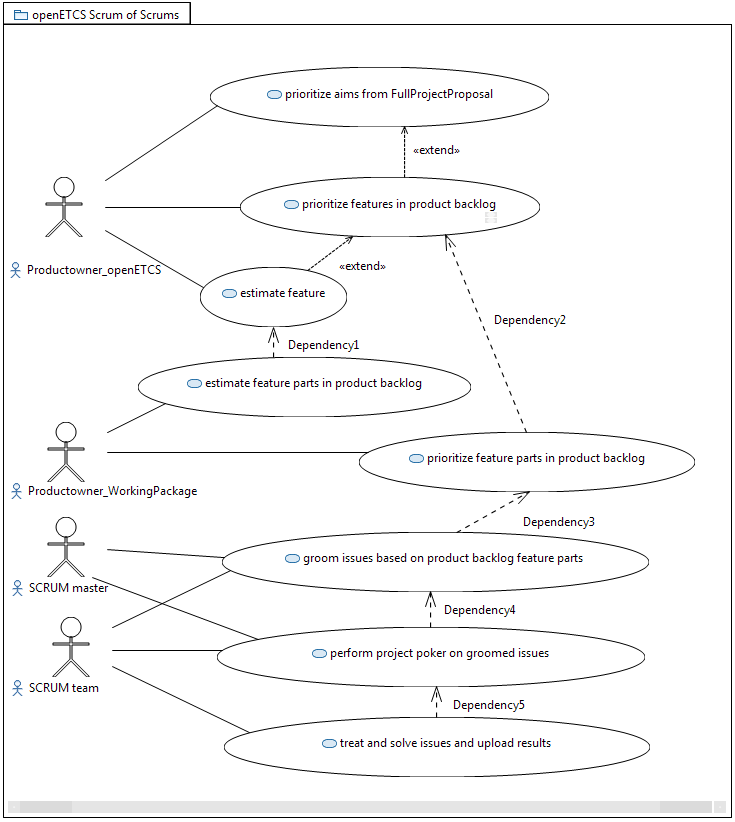
\includegraphics[width=0.7\linewidth]{./images/openETCSVnVScrumOfScrum_02}
\caption{openETCS scrum of scrums}
\label{fig:openETCSVnVScrumOfScrum}
\end{figure}

Within the agile scrum process of openETCS different backlogs are used to synchronise the top level project goals with the tasks performed within the project: 

\begin{itemize}
\item Each backlog itself consists of items which are represented within the github issue tracker. 
\item For each backlog a Product Owner is assigned to coordinate and prioritize the items.
\item Each Story Point (SP) is estimated to be worth one person day.
\end{itemize}


\textbf{The Product Backlog (Product Owner: Klaus-Rüdiger Hase)}
The Product Backlog consists of top level \textit{Features} by which the product is described.
\begin{itemize}
\item  Each Feature itself is estimated by the product owner on how many Story Points this Feature is worth.
\item  A Feature itself is divided into **Feature Parts**.
\item  A Feature Part is related directly to a working package and the repository the work is documented in.
\item  Each Feature Part itself is estimated and prioritized by the product owner on how many Story Points this Feature Part is worth.
\end{itemize}


By estimating the feature the feature becomes accepted on product Level.
The Product Backlog is maintained during a regular meeting.

\textbf{Transferring the Features from the \textit{Product Backlog} to the Verification and Validation Sprint Backlog}
During regular grooming sessions the scrum team extracts the items with highest priority out of the Product Backlog and refines them to issues within the repository mentioned within the Feature Part.
On these issues Project Poker is performed on and by this Story Points are assigned. The decision on which items enter the Sprint Backlog is based on the maximum benefit analysis taking into account the priority as well as the story points.

\textbf{Sprint Backlog}
The \textit{Sprint Backlog} consists of issues which are processed during the Sprint.
During the Sprint the success is tracked against the Sprint Backlog.
The Story Points are earned once the complete result of what has been groomed is uploaded to the github.

\chapter{Release Principals}
\label{sec:Releases}

The agile SCRUM development has an incremental approach dividing the system into smaller functional parts, which are gradually developed and implemented. The model-based development approach using SCADE makes it possible to incorporate all developed parts as soon as possible and thereby making it possible at an early stage to simulate the provided functionality. This continuous development results in releases with reduced functionality, which are in itself consistent and can be used by other SCRUM Design Teams and the V\&V Team to synchronize there functionality or tests.

In this agile development, the incremental delivery quickly allow feedback from the customers, which in the case of openETCS are the project management and other railway stockholders. As an ETCS OBU is a highly safety-relevant system and openETCS is only developing the software kernel the releases cannot be tested in a productive implementation. But the use of simulations and demonstrators allows to address the main functional aspects. In addition the agile development can combine an external delivery of large components of the overall system with frequent and internal deliveries for simulations. Thereby, the internal releases are not following a concrete pre-planed system, but are triggered by the speed of development and the need of other Scrum Teams to access certain functionalities. The SCRUM Teams select the entries from the backlog which are entered in a sprint and define the criteria when a task is done from their perspective. For example in openETCS a model including a defined set of functions is handed over from the design to the V\&V SCRUM Team for independent evaluation and validation of these functions. The V\&V team documents it's findings for all artifacts in their respective reports and gives them as feedback via github issues back at the Design Team.  

Nevertheless, for the overall planning and the interaction with external partners broad milestones are defined in openETCS which are used as a basis for activities which are not performed will modeling the system such as not automatic generated documentation or assessment. This openETCS release interaction between the design and V\&V SCRUM sprints is schematically shown in figure \ref{fig:openETCSReleases}.

\begin{figure}[hbt]
\centering
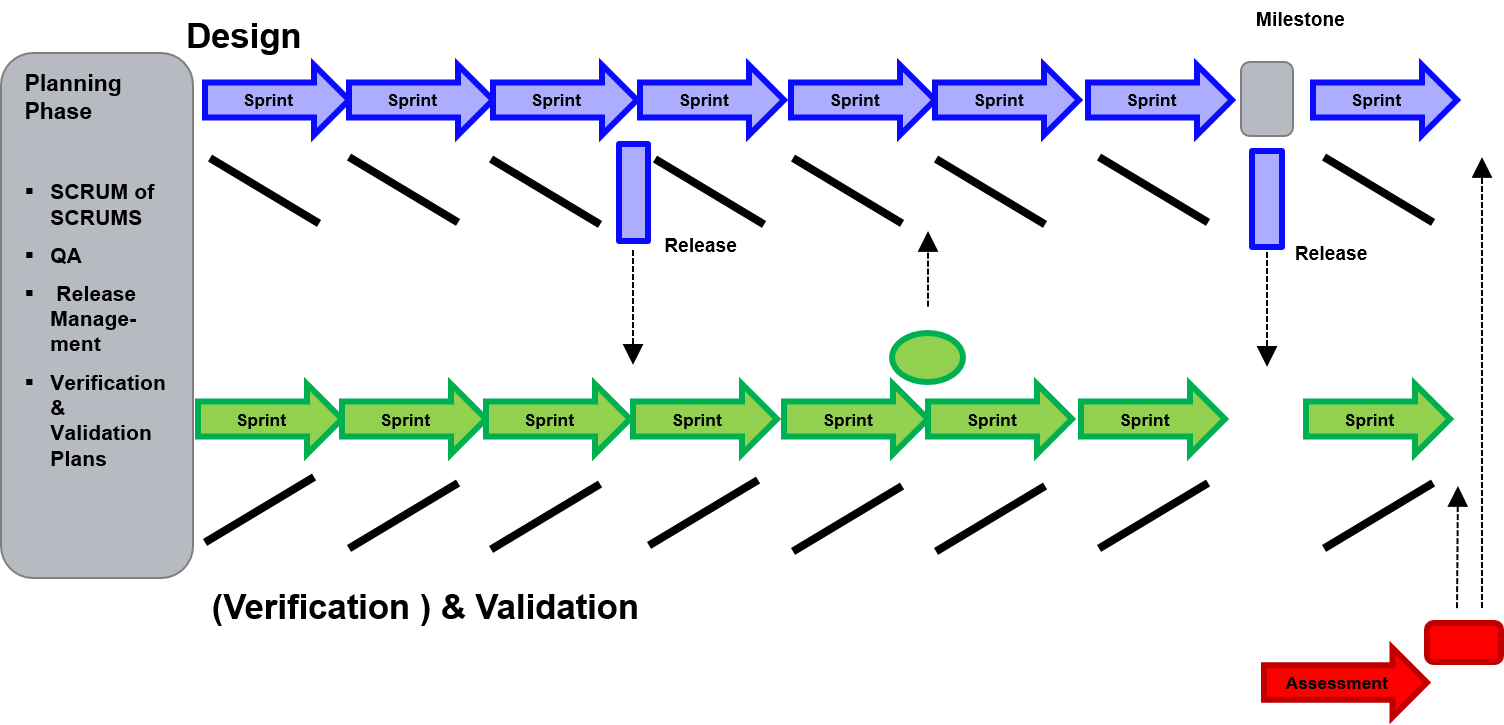
\includegraphics[width=0.95\linewidth]{./images/openETCS_release-concept}
\caption{openETCS release concept}
\label{fig:openETCSReleases}
\end{figure}

As in a SIL 4 development in the end the assessment of all artifacts for the final release have to be reviewed by an authorized independent assessor this phase can not be integrated in the continuous agile process. But ideally the assessor is already involved in the main development and thereby already reaches  preliminary results for long time stable parts of the system. However, the release provided for assessment and afterwards for use has to be a self-sufficient collection which can be reviewed independent of all pre-releases. Since the openETCS project only develops the a functional ETCS OBU it is not providing a release ready for a complete safety assessment. 

\begin{comment}
\chapter{Conclusion}
\label{sec:conclusion}

can be left open for now

final conclusion of content 
\end{comment}

%\bibliographystyle{unsrt} %
%\bibliography{./ref/ref-HaRA}


%===================================================
%Do NOT change anything below this line

\end{document}


